\cotefile{134-2}
\scanpage{170}\mspage{25}%
% archive sheet number: 170
On dira qu'une $n$-catégorie \inserted{$\unsure{\mathcal E|E}_{n}$} est ``\uline{spéciale}'' (ou $n$-\uline{galoisienne}) si elle est $n$-équivalente à la cat. des $(n-1)$-champs loc. constants sur un espace top. (ou un topos) convenable, ou ce qui doit revenir au $\unsure{=|\overline m}$, si elle est $n$-équivalente à la catégorie des $n$-foncteurs $G_n\longrightarrow(n\text{-}\mathrm{Cat})$, où $G_n$ est un $n$-groupoïde, Si $X$, $G_n$, $\mathcal E_n$ se correspondent ainsi, on dit que $\deleted{\unsure{G_n|\mathcal E_n}}\,G_n$ est le $n$-groupoïde fondamental de $X$, ou de $\mathcal E_n$, ou que $\mathcal E_n$ est la catégorie des $n$-systèmes locaux sur $X$, ou sur $G_n$, ou que $X$ est une réalisation géométrique \unsure{de|du} $G_n$ ou de $\mathcal E_n$. En analogie avec le cas bien familier $n=1$, $G_n$ doit s'interpréter comme la sous-$n$-catégorie pleine de $\underline{\mathrm{Hom}}_n(\mathcal E_n,(n\text{-}\mathrm{cat}))$ formée des $n$-foncteurs $\mathcal E_n\to(n\text{-}\mathrm{cat})$ satisfaisant certaines propriétés d'exactitude (on a envie de dire : qui commutent aux $\unsure{\varprojlim|\underline{\lim}}$ finies et aux $\varinjlim$ quelconques) ; mais cela nous
% Faint interlinear curved mark below nous, whole-image x290–318, y1991–2018; hand/function uncertain.
\raisebox{-1.8ex}[0pt][0pt]{\makebox[0pt][r]{\parbox{3mm}{\figure{\begin{tikzpicture}[x=1mm,y=1mm]
\draw[line width=0.25pt,gray] (0,0) .. controls (0.35,-1.15) and (1.55,-2.45) .. (2.2,-2.55) .. controls (2.65,-2.7) and (2.7,-2.2) .. (2.38,-1.85);
\end{tikzpicture}}}}}
 attire dans l'inquiétant engrenage des $n$-limites dans les $n$-catégories (\uline{NB} le cas $n=2$ commence à nous être familier\ldots) Il est prudent dans tout
\scanpage{171}\mspage{26}%
ceci de supposer que $X$ est ``localement homotopiquement trivial'', ce qui assure que le pro-ensemble simplicial que lui associent Artin-Mazur (par le procédé de nerfs de 'hyperrecouvrements) est essentiellement constant dans la catégorie homotopique ordinaire - donc $X$ définit un type d'homotopie habituel. Ce n'est \uline{pas} le cas bien sur pour le topos étale d'un schéma, Pour un tel cas, le $n$-groupoïde fondamental doit être conçu comme un \uuline{pro}-$n$-groupoïde (rien d'étonnant à cela, vu la théorie familière \unsure{du|des} $\pi_1$) ; et $\unsure{\mathcal E|E}_n$ comme une $(\mathrm{ind})$-$n$-catégorie (\unsure{le|la} ind-structure correspondant à l'exigence de locale trivialité, pour un $n$-champ variable, relativement à des recouvrements de plus en plus fins de $X$).

\figure{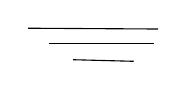
\begin{tikzpicture}[x=1cm,y=1cm]
\draw (0,0)--(1.65,-.01);
\draw (.27,-.19)--(1.60,-.19);
\draw (.57,-.40)--(1.34,-.42);
\end{tikzpicture}}

Je comprends cependant ta résistance instinctive à concevoir ce dépouillement extrême d'un beau topos $X$, au point de%
% Isolated short pen stroke at the right edge, between manuscript baselines 21 and 22; no textual interpretation.
\margin{\figure{\begin{tikzpicture}[x=1cm,y=1cm]\draw[line width=.5pt] (0,0)--(.14,.025);\end{tikzpicture}}}
n'en retenir que le maigre type d'homotopie. Bien plus, je suis persuadé qu'en%
% Isolated small black point at the lower right, below and right of the final n; origin uncertain, not assigned sentence punctuation.
\margin{\figure{\begin{tikzpicture}[x=1cm,y=1cm]\fill (0,0) circle[radius=.018];\end{tikzpicture}}}
% archive sheet number: 171
\scanpage{172}\mspage{27}%
allant jusqu'au bout\unsure{,} de cette résistance à fleur de peau, on arrive à généraliser et à approfondir la notion de ``type d'homotopie'', et à apporter encore une nouvelle eau au développement d'un bon yoga homotopique. Voici où je veux en venir.

Parlons d'abord de faisceaux \inserted{(d'ens, ou de modules etc)}, pour simplifier, au lieu de champs, \inserted{et \unsure{plaçons-nous|plaçons nous} sur le topos étale d'un schéma $X$.} Les faisceaux loc. constants - modulo une condition de finitude supplémentaire assez anodine - forment les plus simples des faisceaux \uline{constructibles}, à la définition desquels ils servent de modèle. Supposant $X$ cohérent ($=$ qu. qct et qu. sép), les faisceaux constructibles généraux sont ceux pour lesquels il existe une partition \inserted{finie} $X=\bigcup\limits_{i\in I}X_i$\raisebox{-1.7ex}[0pt][0pt]{\makebox[0pt][r]{\parbox{1.5mm}{\figure{\begin{tikzpicture}[x=1mm,y=1mm]\fill (0,0) circle[radius=.14];\end{tikzpicture}}}\hspace{.8em}}} de $X$ en ``cellules'' \inserted{ou ``strates''} $X_i$, loc. fermées et constructibles, telles que \deleted{\unsure{chaque|chaq.}} la restriction de $F$ à chaque $X_i$ soit loc constant \deleted{et} (plus une condition de finitude\ldots) Ainsi la catégorie des faisceaux constructibles sur $X$ . (qui redonne la catégorie de tous les faisceaux en passant à une catégorie de ind-objets\ldots) \unsure{apparait|apparaît} elle-$\overline m$ comme limite inductive de catégories, associées à des partitions de plus en
% Small point at whole-image (1161,1361), below/right of the union index: reproduced by the zero-width raised box; no mathematical role is assigned.
% The separate point after X on L20 is reproduced as a physical point, not asserted to end a sentence.
% archive sheet number: 172
\scanpage{173}\mspage{28}%
plus fines de $X$. On peut alors, pour une telle partition \uline{fixée} \inserted{$\unsure{\mathcal P|P}$}, se proposer \unsure{une|d'une} étude approfondie \inserted{de la cat.} des faisceaux (ou complexes de faisceaux, ou champs) qui sont ``$\mathcal P$-constructibles'' (ou plus généralement, qui sont ``loc. constants'' sur chacun des $X_i$). Ces catégories n'auront des structures vraiment \deleted{Pour \unsure{préciser|pouvoir} di} satisfaisantes que si elles sont stables par les opérations courantes - telles que $\mathrm R\underline{\mathrm{Hom}}$, ou $\mathrm Rj_*j^*$ où $j:X_i\mathrel{\unsure{-|\longrightarrow}}X$ est une ``cellule'' de la partition, \inserted{etc}.\raisebox{0.35ex}[0pt][0pt]{\parbox[c][0pt][c]{0pt}{\figure{\begin{tikzpicture}[x=1pt,y=1pt,baseline=0pt]\fill (0,0) ellipse (0.35 and 0.2);\end{tikzpicture}}}} En fait, si $X$ est excellent et qu'on dispose de la résolution des singularités, on sait que les faisceaux \inserted{de torsion} constructibles . (sous réserve d'être premiers aux car résiduelles) sont stables par \deleted{\unsure{toutes|toute}} ces opérations - mais non avec une partition de $X$ fixée une fois pour \unsure{toute|toutes}. Pour avoir une telle stabilité plus fine, il faut faire des hypothèses très strictes \deleted{\unsure{sur}} ``d'équisingularité'' de la stratification donnée de $X$, le long de ses strates. Je pense néanmoins qu'un \unsure{raffinement|affinement} des techniques connues montrera que $X$ admet des stratifications arbitrairement fines ayant ces propriétés d'équisingularité (et avec des $X_i$ réguliers et connexes, mais peu importe \unsure{pour} notre propos \unsure{présent}\ldots). À titre d'exemple
% The cancelled phrase Pour préciser/pouvoir di is physically below structures vraiment (L7), not after que si. No insertion caret makes structures an addition.
% The small TikZ dab is the distinct point above/right of the ordinary point before En fait (whole-image centre approximately 1230,897); its origin is uncertain.
% archive sheet number: 173
\scanpage{174}\mspage{29}%
supposons qu'il y ait exactement deux strates, une strate fermée $X_0$ et $X_1=X-X_0$. D'après le dévissage d'Artin, un faisceau $F$ sur $X$ revient à la donnée d'un faisceau $F_0$ \inserted{$(=i_0^*(F))$} sur $X_0$, d'un faisceau $F_1$ \inserted{$(=i_1^*(F))$} sur $X_1$, et d'un homomorphisme $F_0\longrightarrow i_0^*i_{1*}(F_1)$. Pour que $F$
% Left marginal diagram, beside manuscript line 7 (not parenthesised in the ink).
\reversemarginpar
\margin{\diagram{\resizebox{\linewidth}{!}{\begin{tikzcd}[ampersand replacement=\&,column sep=1.2em]
X_0 \arrow[r,hook,"i_0"] \& X \& X_1 \arrow[l,hook']
\end{tikzcd}}}}%
\normalmarginpar
soit $\unsure{\mathcal P|P}$-constructible, il. f et s. que $F_0$ et $F_1$ soient loc. constants (plus des conditions de finitude accessoires\ldots), sur $X_0$ et $X_1$ respectivement. Alors (grâce aux hyp. d'équisingularités) il en sera de $\overline m$ de $i_0^*i_{1\unsure{*|,}}(F_1)=\varphi(F_1)$, et \inserted{la cat.} des faisceaux qui nous \unsure{intéressent}\deleted{\unsure{s|t}} s'exprime entièrement en \deleted{\unsure{fonction}} \inserted{termes} de catégories de faisceaux loc. constants sur $X_0$ et $X_1$, \deleted{\uline{\unsure{i.e. de la|i.e. de leurs}} \unsure{d}} \inserted{i.e. des \inserted{seuls} types} d'homotopie de $X_0$ et $X_1$, à celà près qu'il faut encore expliciter la nature du foncteur exact à g. $\varphi$. Je pense que ceci est possible, dans le contexte \inserted{\uline{schématique}} où je me suis placé (techniquement assez sophistiqué), en introduisant un ``voisinage tubulaire étale'' de $X_0$ dans $X$ (qui est un topos fort intéressant, mais pas associé à un schéma). Mais cette construction technique ne fait que para%
% The possible cancelled d at L15 may instead be the descender of live types.
% A continuation hyphen follows para at the physical page end; suppressed here for joining the continued word under the brief's convention.
% archive sheet number: 174
\scanpage{175}\mspage{30}%
phraser une intuition topologique extrêmement simple, que je vais expliciter, en supposant pour fixer les idées qu'on est sur le corps de base $\mathbb C$ et qu'on en profite pour travailler avec
% Compact isolated point at whole-image (171,423), left of L5; origin and role uncertain.
\raisebox{0pt}[0pt][0pt]{\parbox{0pt}{\figure{\begin{tikzpicture}[overlay,x=1pt,y=1pt]\fill (-7,0) ellipse[x radius=.35pt,y radius=.5pt];\end{tikzpicture}}}}%
les espaces loc. compacts habituels. L'idée topologique derrière l'hypothèse d'équisingularité, c'est qu'il existe un \uline{voisinage tubulaire $T$} de $X_0$ dans $X$ se rétractant sur $X_0$, et tel que $(X_0,T)$ au dessus de $X_0$ soit un fibré \unsure{loclement|localement} trivial, donc $T-X_0$ au dessus de $X_0$ est loc trivial. En fait, \deleted{\unsure{on pourra con|on pourra cons}} \inserted{si $\partial T$ est le} ``bord'' de $T$, qui sera aussi fibré loc. trivial sur $X_0$, $T$ sur $X$ est le fibré en cônes déduit ($\simeq(\partial T\times I)\amalg_{\partial T}X_0$, où $I=[0,1]$, $\partial T%
% Compact isolated point at whole-image (702,1183), above the first relation shaft; not a mathematical dot.
\raisebox{1.3ex}[0pt][0pt]{\parbox{0pt}{\figure{\begin{tikzpicture}[overlay,x=1pt,y=1pt]\fill (4,0) -- (4.7,.6) -- (4.8,-.5) -- cycle;\end{tikzpicture}}}}%
\mathrel{\to}\partial T\times I$ défini par $x\mathrel{\unsure{\mapsto|\vdash}}(x,1)$, et $\partial T\mathrel{\unsure{-|\to}}X_0$ est la projection) donc $\mathring T=T-X_0\simeq\partial T\times[0,1[$ est $X_0$-homotope à $\partial T$. Si $X_0$ et $X_1$ sont non singuliers, il en est de $\unsure{=|\overline m}$ de $\mathring T$ et $\partial T$, qui sont des fibrés topologiquement lisses sur $X_0$. D'ailleurs, $\deleted{\unsure{X_1|X}}$ posant $\widetilde X_1=X_1-\mathring T$, \deleted{$\unsure{\widetilde X_1|X_1}$ dev.} l'inclusion $\widetilde X_1%
% Short isolated dark tick at whole-image (259,1797), below this source object; origin and role uncertain.
\raisebox{-2.3ex}[0pt][0pt]{\parbox{0pt}{\figure{\begin{tikzpicture}[overlay,x=1pt,y=1pt]\draw[line width=.55pt] (0,.6) -- (.2,-.6);\end{tikzpicture}}}}%
\hookrightarrow X_1$ est une équivalence d'homotopie, et $X$ se réconstitue, à homéomorphisme près, à partir \unsure{du|des} diagramme d'espaces
\diagram{\begin{tikzcd}[ampersand replacement=\&,column sep=small,row sep=large]
(\mathring T=T-X_0\underline{\approx}) \& \partial T \arrow[r,"\unsure{J|j}","\text{inclusion}"'] \arrow[d,"p","\text{fibration}"'] \& \widetilde X_1\,(\underline{\approx}X_1)\\
\& X_0 \&
\end{tikzcd}}
comme la somme amalgamée. En termes de ce diagramme d'espaces; le foncteur $\varphi$ plus
% archive sheet number: 175
\scanpage{176}\mspage{31}%
haut s'interprète immédiatement comme
\[
\varphi(F_1)\simeq p_*{\unsure{J|j}}^*(\widetilde F_1)
\]
où $F_1\mapsto\widetilde F_1$ est la restriction de $X_1$ à $\widetilde X_1$ (qui
est donc une équivalence de catégories pour les
faisceaux (loc. const.) envisagés). \deleted{\unsure{Il|Il s'|\ensuremath{J}} \unsure{peut|peut se|\ensuremath{J^*}}} \inserted{La donnée}
d'un\inserted{\unsure{e}} $F=(F_0,F_1,u:F_0\to\varphi F_1)$ peut donc aussi
s'expliciter comme la donnée de
\[
F_0,\ \widetilde F_1,\ \widetilde u:p^*(F_0)\longrightarrow J^*(\widetilde F_1)
\]
où $F_0$ ($\widetilde F_1$) est un faisceau loc. constant sur
$X_0$ (resp. $\widetilde X_1$). Il faut se rappeler de plus
qu'ici $p$ est une vraie fibration, et $J$ une inclusion
(et pratiquement, -- cas $X_0,X_1$ lisses --
\deleted{\unsure{une}} l'inclusion du bord dans une variété
à bord).

Si on préfère, on peut aussi prendre le
diagramme un peu moins joli (mais un
peu plus canonique)
\diagram{\begin{tikzcd}[ampersand replacement=\&,column sep=large,row sep=large]
\mathring T \arrow[r,"J'"] \arrow[d,"p'"] \& X_1\\
% Small isolated dark stroke at whole-image (353,1845), about 380 px left of X_0.
% Its origin is uncertain; it is not punctuation or a mathematical symbol.
\raisebox{0pt}[0pt][0pt]{\parbox{0pt}{\figure{\begin{tikzpicture}[overlay]
\fill (-40mm,0.8mm) .. controls (-39.7mm,0.6mm) and (-39.8mm,0.35mm) .. (-39.7mm,0.05mm)
-- (-40.1mm,0.1mm) .. controls (-40.2mm,0.35mm) and (-40mm,0.45mm) .. (-40.1mm,0.7mm) -- cycle;
\end{tikzpicture}}}}X_0 \&
\end{tikzcd}}
revenant essentiellement au $\overline m$, car formé d'espaces
homotopes au précédent. On peut $\overline m$ y remplacer
$X_0$ par $T$ ($X_0$ en étant un rétract par déformation) et écrire
\diagram{\begin{tikzcd}[ampersand replacement=\&,column sep=large,row sep=large]
\mathring T \arrow[r,hook,"J'"] \arrow[d,hook,"p''"] \& X_1\\
\unsure{T|I} \&
\end{tikzcd}}
% archive sheet number: 176
% The bottom target is cut close to the paper edge; no content supplied from another page.
\scanpage{177}\mspage{32}%
% archive sheet number: 177
où ``pris à la lettre'' $p''$ est maintenant une inclusion, mais ``moralement'' c'est \inserted{tjrs} une fibration à fibres très \unsure{polies|jolies} [de dim finie notamment, voire des variétés non singulières - c'est donc beaucoup mieux que ce que nous donne le yoga de Cartan-Serre ``toute application continue est équivalente à une fibration''\ldots] C'est ce dernier diagramme qui est susceptible d'une construction directe, purement algébrique, dans le cadre des schémas, lorsque l'on a développé la construction du voisinage tubulaire étale.

Le point où je veux en venir, c'est que la considération \inserted{de la cat} des faisceaux (ou \inserted{complexes d'iceux, ou} $n$-champs \unsure{..|\ldots}) $\unsure{\mathcal P|P}$-constructibles sur un $X$, où $\mathcal P$ est une stratification ``équisingulière'' donnée\raisebox{0pt}[0pt][0pt]{\parbox{0pt}{\figure{\begin{tikzpicture}[overlay,x=1mm,y=1mm]\fill (-6,-1.5) circle[radius=.12mm];\end{tikzpicture}}}}, revient dans le cas particulier actuel à la connaissance d'un diagramme de \uline{types d'homotopie}\raisebox{0pt}[0pt][0pt]{\parbox{0pt}{\figure{\begin{tikzpicture}[overlay,x=1mm,y=1mm]\fill (6,.8) ellipse[x radius=.08mm,y radius=.19mm];\end{tikzpicture}}}} \inserted{(ou de pro-types, si on revient à la top. étale)}\raisebox{0pt}[0pt][0pt]{\parbox{0pt}{\figure{\begin{tikzpicture}[overlay,x=1mm,y=1mm]\draw[line width=.2pt] (2.4,1.15) -- (2.5,.7);\end{tikzpicture}}}} ordinaires
% The parenthesis is physically above ordinaires, without an attachment guide.
% Its visible order before ordinaires is retained; ordinaires is not marked as an insertion.
% Nontext marks above: (1158,1368) below donnée; (1633,1538) right of underline;
% (1333,1563) just above/right of the parenthesis. Presence is clear; origin is uncertain.
\diagram{\begin{tikzcd}[ampersand replacement=\&,column sep=large,row sep=large]
\unsure{\Delta|\triangle} \arrow[r,"\unsure{J|j}"] \arrow[d,"p"'] \& X_1\\
X_0 \&
\end{tikzcd}}
\raisebox{0pt}[0pt][0pt]{\parbox{0pt}{\figure{\begin{tikzpicture}[overlay,x=1mm,y=1mm]\draw[line width=.3pt] (8,4.4) -- (8.05,4.2) -- (8,4);\end{tikzpicture}}}}en prenant des systèmes de coeff locaux (ou de $n$-champs loc. constants) sur ces sommets \inserted{$X_0,X_1$ \deleted{$\unsure{\Delta|X}$}} reliés par des hom de \unsure{compatibilité|compatibilit} du type $p^*(F_0)\to J^*\unsure{(}F_1)$. Ce serait un exercice amusant (que je n'\unsure{ai} pas encore fait) de
% The isolated short dark mark at (315,1849), above prenant, has uncertain origin.
% The crossed triangular sign is in the insertion above the gap after sommets;
% the tall live l of reliés passes into the same crowded area.
% The manuscript stops at the complete word de; no following text is supplied.
\scanpage{178}\mspage{33}%
vérifier et d'expliciter comment les ``6 opérations'' habituelles sur les faisceaux (soit sur $X$, soit sur une réunion de strates de $X$) peuvent s'exprimer dans ce dictionnaire, dans le cas disons de strates non singulières (\unsure{autrement}, on aurait des difficultés avec les complexes dualisants, dont on aimerait qu'ils appartiennent à notre catégorie%
% A pale isolated point at approximately (949,661), below the aligned ellipsis deposits; origin uncertain, no punctuation function assigned.
\raisebox{0pt}[0pt][0pt]{\parbox{0pt}{\figure{\begin{tikzpicture}[overlay]\fill[black!45] (0,-0.06) circle[radius=0.018cm];\end{tikzpicture}}}}%
\unsure{.\,.\,.\,.\,.|\ldots}) \inserted{et de revérifier le formulaire connu de ces opérations}. Mais il apparaitra probablement que, pour bien pouvoir tout transcrire, il convient, plutôt \inserted{que} de regarder un diagramme du type
\diagram{\begin{tikzcd}[ampersand replacement=\&,column sep=1.4em,row sep=1.2em]
\cdot \arrow[r] \arrow[d] \&
% Distinct off-axis point at approximately (1229,905), below/right of the right arrowhead; it is not a target object. Its origin is uncertain.
\raisebox{0pt}[0pt][0pt]{\parbox{0pt}{\figure{\begin{tikzpicture}[overlay]\fill (0.16,-0.15) circle[radius=0.018cm];\end{tikzpicture}}}} \\
{} \& {}
\end{tikzcd}}
dans la catégorie homotopique formée avec la cat.\,. des ens. semi-simpliciaux, \inserted{de} regarder la catégorie des diagrammes d'ensembles $1/2$ simpliciaux, et à partir de là passer%
% Small isolated point at approximately (1359,1333), below the latter part of passer; origin uncertain.
\raisebox{0pt}[0pt][0pt]{\parbox{0pt}{\figure{\begin{tikzpicture}[overlay]\fill (-0.35,-0.15) circle[radius=0.016cm];\end{tikzpicture}}}} à une catégorie homotopique de %
% Isolated point at approximately (1157,1368), above/left of the f of fractions; origin uncertain.
\raisebox{0pt}[0pt][0pt]{\parbox{0pt}{\figure{\begin{tikzpicture}[overlay]\fill (0,0.37) circle[radius=0.022cm];\end{tikzpicture}}}}fractions.

J'ai plus ou moins explicité dernièrement, en cogitant sur \deleted{\unsure{les|des|ces}}des fondements de ``topologie modérée'' (i.e. où on élimine d'emblée tous les phénomènes de sauvagerie), comment une stratification équisingulière%
% Cancelled interlinear parenthesis above équisingulière; the enclosing/attachment stroke reaches the destination just before the comma.
\inserted{\deleted{(d'un espace \unsure{modéré} \unsure{compact})}}, à strates non singulières disons, d'un ``espace modéré'' \inserted{compact}, donne naissance canoniquement à un diagramme \deleted{\unsure{fon|f}} d'espaces,
% archive sheet number: 178
\scanpage{179}\mspage{34}%
% archive sheet number: 179
qui sont des variétés à bord, les \deleted{\unsure{morp|morph}} flèches des
diagramme étant pour l'essentiel des fibrations
loc. triviales de variétés à bord sur d'autres
(à fibres des variétés à bord), \uline{et} \deleted{\unsure{des|les}}\unsure{les|des} inclusions
des bords dans les variétés à bord \deleted{(}[en
fait, on trouve des inclusions légèrement
plus générales, certains des bords qui apparaissent
étant munis d'une décomposition
cellulaire ``élémentaires'', \deleted{en \unsure{cellules|éléments}}\inserted{i.e. dont \unsure{toutes}} les
% L9: the live replacement runs above the cancelled baseline; toutes is raised with it.
strates \inserted{fermées} sont encore des variétés à bord qui se
recollent suivant des parties communes du
bord~; et il y a lieu d'envisager \inserted{aussi} les inclusions
de ces morceaux les uns dans les
autres\ldots.\deleted{)}], et se réconstitue à partir de
ce diagramme \inserted{par recollement}. En d'autres termes, on
a une description-dévissage canonique
des espaces modérés compacts \inserted{$X$}, éventuellement
munis de stratifications équisingulières
à strates non sing., en termes de diagrammes
\inserted{\unsure{finis}} de nature \unsure{précisé|précisée} formés avec des variétés
à bord. Quand on s'intéresse aux faisceaux
\inserted{(ou complexes de faisceaux, ou $n$-champs\ldots)}
$\unsure{\mathcal{P}|P}$-constructibles sur $X$, où $\mathcal{P}$ est une telle
stratification fixée, ceux-ci s'explicitent en
termes du diagramme envisagé, dont il
\scanpage{180}\mspage{35}%
% archive sheet number: 180
% C original page filename: codex/H134-06/pages/H134-06_134-2_scan180.tex
n'y a plus lieu de retenir que le ``type d'homotopie''. On prévoit que les 6 opérations sur ces faisceaux peuvent se traduire ad-hoc dans ce cadre homotopique. Enfin, si au lieu d'un seul espace modéré compact $X$, on a disons un morphisme modéré $f:X\mathrel{\unsure{-|\to}}Y$ de tels, alors, choisissant des stratifications équisingulières sur $X$ et $Y$ adaptées à $f$ (les strates de $X$ étant notamment des fibrés loc triviaux sur celles de $Y\ldots$), on doit trouver un ``morphisme'' du diagramme de variétés à bord exprimant
% L12: distinct inline point at about (854,1096), just beyond X; origin and sentence role unassigned.
$X$. dans celui exprimant $Y$ (avec des morphismes \unsure{virtuels|mutuels} se ramenant \deleted{\unsure{a|à|,}} encore, pour l'essentiel, à des fibrations de variétés à bord sur d'autres) de telle façon que les 4 opérations $\mathrm{R}\deleted{\unsure{f}}g_*$, $\mathrm{R}g_!$, $\mathrm{L}g^*$,
% L16: isolated nontext slant at about (1327,1557)--(1332,1564), below and left of the fourth operation; origin uncertain.
$g^!\raisebox{0pt}[0pt][0pt]{\parbox{0pt}{\figure{\begin{tikzpicture}[overlay]\draw[line width=0.3pt] (-0.45,-0.34)--(-0.41,-0.42);\end{tikzpicture}}}}$ entre faisceaux \inserted{$\unsure{\mathcal{P}|P}_X$- et $\mathcal{P}_Y$-constructibles} sur $X$ et $Y$ (ou sur des sous-espaces loc. fermés \inserted{$X'$, $Y'$} réunions de strates, de sorte que $f$\unsure{,|.} induise $g:X'\mathrel{\unsure{-|\to}}Y'$) s'expriment encore en termes d'opérations standart entre seuls types d'homotopie.
% L21: two distinct nontext points at about (1000,1994) and (996,2001), above the first stroke of Enfin; origin uncertain.
\raisebox{0pt}[0pt][0pt]{\parbox{0pt}{\figure{\begin{tikzpicture}[overlay]\fill (0.13,0.76) circle (0.010);\fill (0.09,0.69) circle (0.010);\end{tikzpicture}}}}Enfin, toutes ces constructions, encore partiellement hypothétiques (y a du travail \inserted{de fondements} sur la planche!) doivent
\scanpage{181}\mspage{36}%
% archive sheet number: 181
% One continuous running paragraph; author number at top centre, archive pencil number at lower left.
pouvoir se paraphraser dans le cadre des schémas excellents, à grands coups de voisinages tubulaires étales.
Dans l'un et l'autre cas, le ``type d'homotopie fin'' d'un espace modéré, resp. d'un schéma excellent, se définirait par passage à la limite à partir des
% L7a: the opening quotation marks stand to the left of the raised prefix; its guide reaches the start of types.
``\inserted{$\unsure{\mathcal{P}|P}$-}types d'homotopie'' associés à des stratifications équisingulières (à strates non sing.) $\mathcal{P}$ de plus en plus fines.
Ce type d'homotopie \inserted{``fin''} incarnerait la connaissance, non des seuls faisceaux ou \inserted{$n$-}champs \unsure{loc.|loc} constants, mais
% L12a: complete interlinear parenthesis; the long guide descends before la.
\inserted{(via un passage à la limite \unsure{inductive})} la connai%
% L12 nontext point at approximately (714,1189), below the ai region; origin uncertain.
\raisebox{0pt}[0pt][0pt]{\parbox{0pt}{\figure{\begin{tikzpicture}[overlay,x=1cm,y=1cm]\fill (-0.04,-0.28) circle (0.35pt);\end{tikzpicture}}}}%
ssance de
% The visible rule begins within the o of tous, approximately (1171,1167), and ends near (1289,1164).
t\uline{ous}. Et il dépendrait, en un sens convenable,
fonctoriellement%
% L14 nontext point at approximately (700,1366), below/right of fonctoriellement; origin uncertain.
\raisebox{0pt}[0pt][0pt]{\parbox{0pt}{\figure{\begin{tikzpicture}[overlay,x=1cm,y=1cm]\fill (0.16,-0.12) circle (0.3pt);\end{tikzpicture}}}}
de $X$. Dans%
% L14 nontext point at approximately (1170,1369), below the end of Dans; origin uncertain.
\raisebox{0pt}[0pt][0pt]{\parbox{0pt}{\figure{\begin{tikzpicture}[overlay,x=1cm,y=1cm]\fill (0,-0.27) circle (0.45pt);\end{tikzpicture}}}}
le cas d'un%
% L14 nontext point at approximately (1627,1352), below/right of d'un, near the right margin; origin uncertain.
\raisebox{0pt}[0pt][0pt]{\parbox{0pt}{\figure{\begin{tikzpicture}[overlay,x=1cm,y=1cm]\fill (0.45,-0.13) circle (0.25pt);\end{tikzpicture}}}}
schéma de type fini sur un corps alg. clos disons, les
% Literal ruled span: from within the é of théorèmes, approximately (671,1580), to (1328,1557), before cohomologique.
th\uline{éorèmes de finitude} cohomologique ou homotopique les plus forts s'exprimeraient précisément en termes des types d'homotopie fin, et diraient que les types d'homotopie \unsure{ordinaire|ordïnaire} qui en sont les élément constituants sont essentiellement des ``\unsure{polyédres|polyèdres} finis'' -- et $\overline{m}$ des variétés à bord compactes -- ou de façon plus précise,
% C original page filename: codex/H134-06/pages/H134-06_134-2_scan182.tex
\scanpage{182}\mspage{37}%
% archive sheet number: 182
% L1a: raised parenthesis, with a long attachment guide entering after profinis.
les ``complétés profinis'' \inserted{(au sens d'Artin-Mazur)} premiers à $p$ (la car. de $k$) de tels espaces.
On voit clairement comment \unsure{aborder} un tel programme en car. $0$, mais on prévoit de l'amusement supplémentaire, voire du mystère, en car $p>0$, pour les variétés qui, même birationnellement, refuseraient de se laisser remonter en car. $0$!

% Separate rule: whole-image endpoints approximately (688,720) and (976,715).
\figure{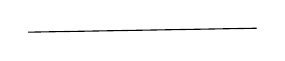
\begin{tikzpicture}
\draw[line width=0.4pt] (0,0) -- (2.9,0.05);
\end{tikzpicture}}

De ces cogitations essentiellement géométriques, je ne saurais à l'heure actuelle tirer un programme précis de développement de structures algébriques adéquates pour les exprimer.
Je me bornerai à quelques remarques en marge.

\deleted{\unsure{a|$\alpha$})} Depuis longtemps j'ai été \unsure{intrigu-|intrigué} par l'idée d'une ``linéarisation'' d'un type d'homotopie (ordinaire), i.e. la question du type: Si $X$ est un type d'homotopie, combien d'information cohomologique du type: cohomologie de $X$ à coefficients variables $M$ (constant%
% Compact detached point near (818,1807), below the first constant; physical presence retained, origin unassigned.
\raisebox{0pt}[0pt][0pt]{\parbox{0pt}{\figure{\begin{tikzpicture}[overlay,x=1pt,y=1pt]
\fill (-28,-7) circle[radius=0.35pt];
\end{tikzpicture}}}} ou constant tordus),
% A detached short vertical mark at approximately (271,1837), above the beginning of structure; origin uncertain.
\raisebox{2.2ex}[0pt][0pt]{\parbox{0pt}{\figure{\begin{tikzpicture}[overlay]
\draw[line width=0.3pt,line cap=round] (0.16,0) -- (0.17,-0.04) -- (0.17,-0.06) -- (0.18,-0.06);
\end{tikzpicture}}}}structure multiplicative
% The two short overwritten strokes favour = over +; the underlying sign remains doubtful.
% A distinct compact point at approximately (1024,1876), below the first H crossbar, is drawn without assigning it a mathematical role.
$\deleted{\unsure{=|+}}\raisebox{0pt}[0pt][0pt]{\parbox{0pt}{\figure{\begin{tikzpicture}[overlay]
\fill (0.09,0.05) ellipse [x radius=0.012cm,y radius=0.02cm];
\end{tikzpicture}}}}H^i(X,M)\times H^j(X,N)\mathrel{\unsure{\dashv|\to|-}}H^{\unsure{i\cdot j|i+j|ij}}(X,M\otimes N)$,
plus éventuellement d'autres opérations cohomologiques -- est-il%
% Detached short hooked stroke at approximately (1619,2077), well to the right of est-il; no word or punctuation function assigned.
\raisebox{0.4ex}[0pt][0pt]{\parbox{0pt}{\figure{\begin{tikzpicture}[overlay]
\draw[line width=0.3pt,line cap=round] (0.25,0) -- (0.27,-0.07) -- (0.31,-0.12);
\draw[line width=0.3pt,line cap=round] (0.27,-0.05) -- (0.26,-0.09);
\end{tikzpicture}}}} nécessaire d'avoir pour \unsure{réconstituer|rêconstituer} le type d'homotopie entièrement \deleted{\unsure{?}}? (disons,
\scanpage{183}\mspage{38}%
% archive sheet number: 183
% One continuous running-prose block; no visible paragraph indent or extra gap at Une fois.
dans cette première approche pré-catégorie dérivée, par la connaissance du groupe fondamental $\pi_1$, donc des catégories des coeff. \unsure{constant|constants} tordus $=\pi_1$-\unsure{module|modules}, les foncteurs
% L5: the argument separator has a high point (about 344,446) and a separate lower comma-shaped stroke.
% Preferred semicolon; alternative comma with an unassigned detached point. Neither element is omitted.
$H^i(-\unsure{;|,}M)$ sur ceux-ci avec \unsure{le|la} structure de \unsure{foncteur|foncteurs} \deleted{\unsure{ab|ab.}, de \unsure{foncteur|foncteurs}} \inserted{\unsure{cohomologique|cohomologiques}} relatif aux suites exactes, \unsure{le|la} \deleted{\unsure{struc}}structure de cup-produit etc --\raisebox{0pt}[0pt][0pt]{\parbox{0pt}{\figure{\begin{tikzpicture}[overlay,x=1em,y=1em]\fill (-0.55,-0.60) circle[radius=0.045em];\end{tikzpicture}}}} reliés par certaines propriétés formelles. Une fois qu'on dispose du langage des cat. dérivées, la \inserted{sous catégorie de la catégorie dérivée des} complexes abéliens, \unsure{formee|forme|formée|form-} \inserted{aux complexes de} faisceaux de coh. loc constante sur $X$, avec sa structure triangulé et sa structure \deleted{\unsure{m|sou|de}}multiplicative
% L13: detached compact point below tensor, approximately (1165,1373); origin and function unassigned.
$\overset{\mathbb{L}}{\otimes}\raisebox{0pt}[0pt][0pt]{\parbox{0pt}{\figure{\begin{tikzpicture}[overlay,x=1em,y=1em]\fill (-0.45,-0.95) ellipse[x radius=0.05em,y radius=0.07em];\end{tikzpicture}}}}$ (et éventuellement $\mathbb{R}\mathrm{Hom}$ \ldots) donnant un candidat plus satisfaisant pour espérer récupérer le type d'homotopie. Je n'ai guère d'idée
% L17: separate short stroke below si (about 241,1836); two compact spots beside ils/permettent
% (about 802,1786 and 874,1810) have unassigned origin, irrespective of their colour.
si\raisebox{0pt}[0pt][0pt]{\parbox{0pt}{\figure{\begin{tikzpicture}[overlay,x=1em,y=1em]\draw[line width=0.6pt] (-0.45,-0.80) -- (-0.42,-0.87) -- (-0.45,-0.90) -- (-0.40,-0.97) -- (-0.37,-0.96);\end{tikzpicture}}}} oui ou non ils\raisebox{0pt}[0pt][0pt]{\parbox{0pt}{\figure{\begin{tikzpicture}[overlay,x=1em,y=1em]\fill (0.08,0.58) circle[radius=0.04em];\end{tikzpicture}}}} \raisebox{0pt}[0pt][0pt]{\parbox{0pt}{\figure{\begin{tikzpicture}[overlay,x=1em,y=1em]\fill (-0.12,0.05) ellipse[x radius=0.055em,y radius=0.07em];\end{tikzpicture}}}}permettent de le récupérer \inserted{en effet}, mais par \raisebox{0pt}[0pt][0pt]{\parbox{0pt}{\figure{\begin{tikzpicture}[overlay,x=1em,y=1em]\fill (-0.10,-0.92) circle[radius=0.045em];\fill (0.06,-0.67) ellipse[x radius=0.045em,y radius=0.06em];\end{tikzpicture}}}}contre n'ai guère de doute qu'en allant au bout de la ``linéarisation'', c'est à dire en partant dans le
% L21 underline: first physical stroke about (318,2273)--(556,2261), second about (581,2262)--(673,2264).
% The first rule begins inside n: a short overlay preserves its terminal covered extent.
% The gap lies mainly under l; another short overlay preserves the second rule's beginning under l's terminal extent.
n\raisebox{0pt}[0pt][0pt]{\parbox{0pt}{\figure{\begin{tikzpicture}[overlay,x=1em,y=1em]\draw[line width=0.35pt] (-0.28,-0.16) -- (0,-0.16);\end{tikzpicture}}}}\uline{on abé}l\raisebox{0pt}[0pt][0pt]{\parbox{0pt}{\figure{\begin{tikzpicture}[overlay,x=1em,y=1em]\draw[line width=0.35pt] (-0.10,-0.16) -- (0,-0.16);\end{tikzpicture}}}}\uline{ien} et travaillant avec la $(n+1)$-catégorie (\unsure{sans|sa|san} \unsure{structures|structure} \unsure{supplémentaires|supplémentaire} dessus!) des $n$-champs loc. constants\raisebox{0pt}[0pt][0pt]{\parbox{0pt}{\figure{\begin{tikzpicture}[overlay,x=1em,y=1em]\fill (0.08,0.62) circle[radius=0.04em];\end{tikzpicture}}}}
% L23: inner doubt concerns sur, not the clear X. The outer doubt concerns the insertion state.
% A curved guide attaches before pour; cancellation/older superposed ink remains a state alternative.
\unsure{\inserted{\unsure{sur} $X$}} pour tout $n$
